
Multimodal machine learning,
which integrates diverse data types
such as audio, video, text, and sensor readings,
has significantly advanced applications
in autonomous systems, healthcare, human-computer interaction,
and smart environments~\cite{He2024Multimodal,Chen2023Dialog,Ang2024Temporal,Wang2023Customer,Hu2021Identifying,Bano2024FedCMD,Yin2023Hybrid,zhao-etal-2021-missing,redcore}.
While the ability to leverage multiple modalities enhances predictive performance and robustness,
real-world deployment often faces critical challenges
with missing modality data,
particularly in safety-sensitive and resource-constrained environments.
In autonomous driving and distributed IoT networks,
for instance,
models must maintain reliable performance
despite incomplete or degraded inputs,
making robust handling of missing modalities
essential for practical deployments.
Missing modality data manifests in two forms:
\emph{partially missing},
where fragments of a modality are lost, for example, missing words in a sentence,
and \emph{fully missing},
where an entire modality becomes unavailable,
for example, complete sensor failure.
The latter presents a substantial challenge,
as standard multimodal models
typically depend on the joint availability of modalities
for accurate predictions.
During inference,
missing modalities can significantly degrade performance,
particularly when different modalities
contribute unequally to the decision-making process.
This degradation is especially problematic
in real-world applications
where retraining models or maintaining multiple variants
is often infeasible due to computational and deployment constraints.

Understanding how modalities interact
is crucial for effective missing modality reconstruction.
As illustrated in Figure~\ref{fig:info_types},
modalities can share \emph{mutual information}
that reinforces predictions,
provide \emph{complementary information}
unique to each modality,
exhibit \emph{contrastive relationships}
that may introduce conflicting signals,
or demonstrate \emph{imbalanced contributions}
where one modality dominates others~\cite{%
	wang2020makes,Peng2022Balanced,%
	hazarika2022analyzing,geraghty2023understanding,redcore}.
These interaction patterns influence how effectively
missing modality data can be reconstructed,
particularly when leveraging remaining modalities
to generate missing features.
\begin{figure}[b!]
    \centering
    \begin{subfigure}[b]{0.24\textwidth}
        \centering
        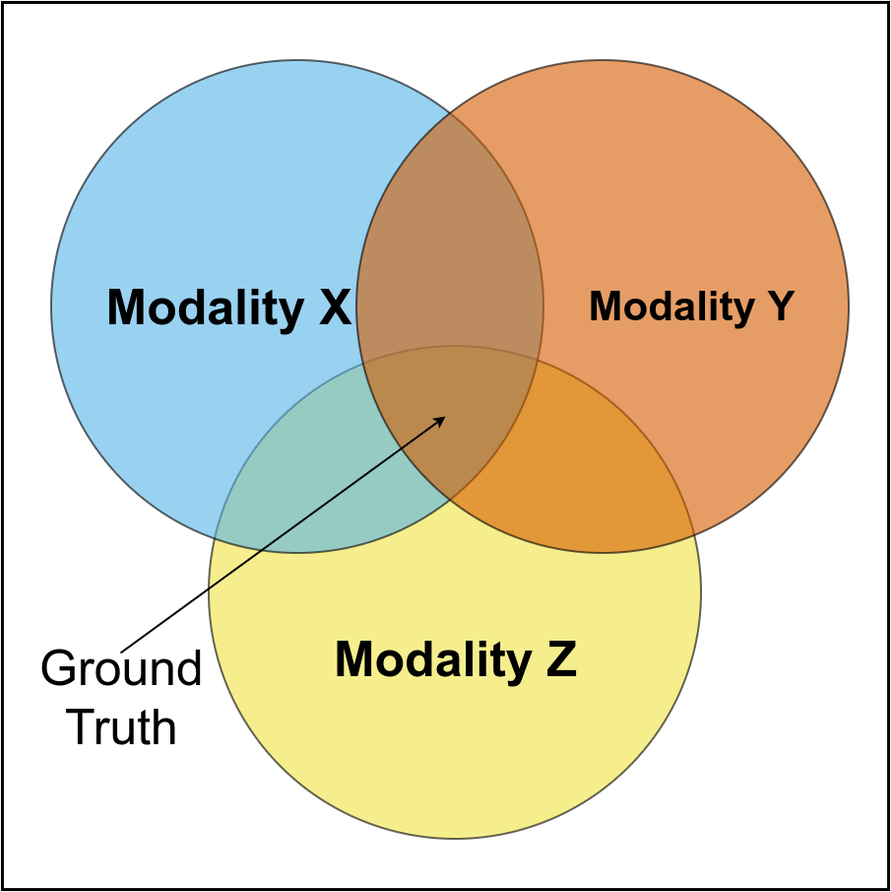
\includegraphics[height=1in]{imgs/mutual_info.png}
        \caption{Mutual Information}
        \label{fig:mutual}
    \end{subfigure}
    \hfill
    \begin{subfigure}[b]{0.24\textwidth}
        \centering
        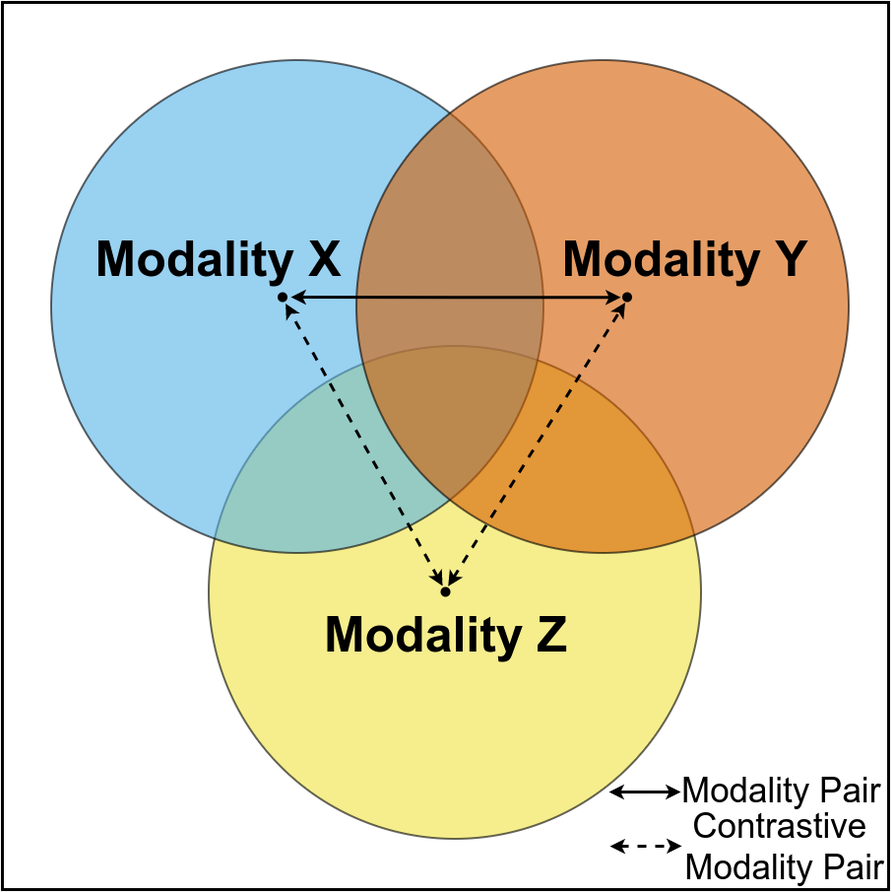
\includegraphics[height=1in]{imgs/complementary_info.png}
        \caption{Complementary Information}
        \label{fig:complementary}
    \end{subfigure}
    \hfill
    \begin{subfigure}[b]{0.24\textwidth}
        \centering
        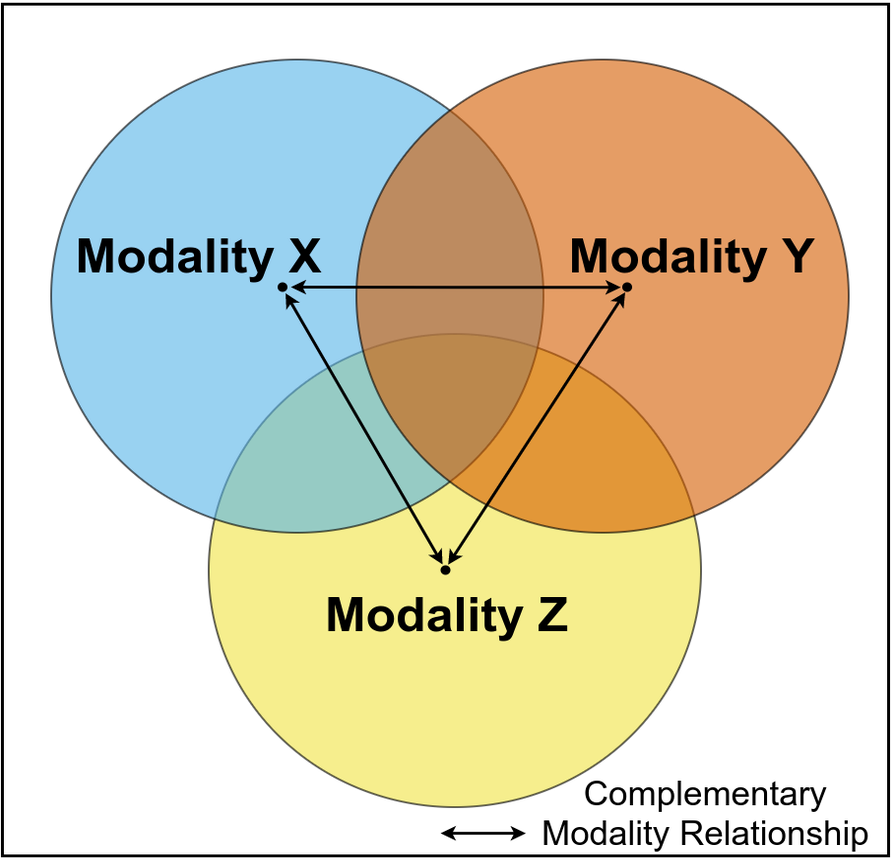
\includegraphics[height=1in]{imgs/contrastive_info.png}
        \caption{Contrastive Information}
        \label{fig:contrastive}
    \end{subfigure}
    \hfill
    \begin{subfigure}[b]{0.24\textwidth}
        \centering
        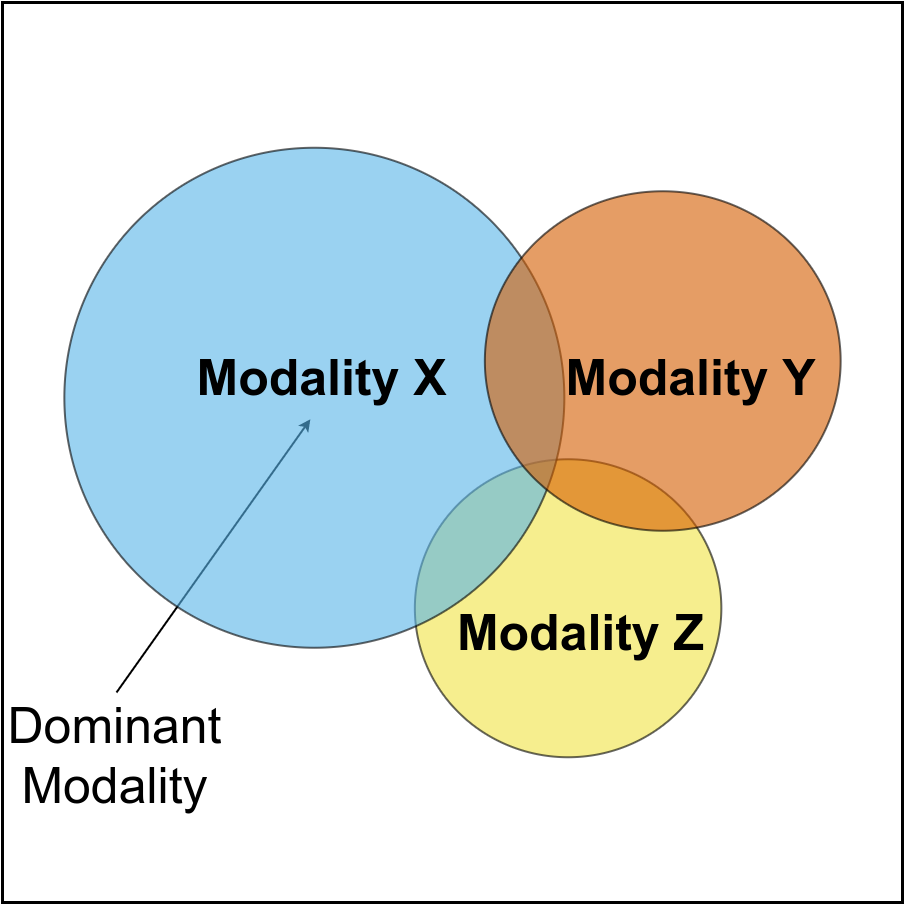
\includegraphics[height=1in]{imgs/imbalanced_info.png}
        \caption{Imbalanced Information}
        \label{fig:imbalanced}
    \end{subfigure}
    
    \caption{%
        Types of information interactions between modalities. 
        \textbf{(a)} Mutual information: Shared knowledge between modalities reinforces predictions.
        \textbf{(b)} Complementary information: Unique knowledge from each modality contributes to the overall task.
        \textbf{(c)} Contrastive information: Modalities provide conflicting signals, which may challenge fusion.
        \textbf{(d)} Imbalanced information: One modality dominates, suppressing the contribution of others.
        Understanding these relationships is critical for effective multimodal learning, particularly when handling missing modalities.
    }
    \label{fig:info_types}
    \Description{Types of information interactions between modalities. 
        \textbf{(a)} Mutual information: Shared knowledge between modalities reinforces predictions.
        \textbf{(b)} Complementary information: Unique knowledge from each modality contributes to the overall task.
        \textbf{(c)} Contrastive information: Modalities provide conflicting signals, which may challenge fusion.
        \textbf{(d)} Imbalanced information: One modality dominates, suppressing the contribution of others.
        Understanding these relationships is critical for effective multimodal learning, particularly when handling missing modalities.}
\end{figure}

Existing approaches for handling missing modalities
primarily intervene during training,
either through generative methods
that learn joint distributions
over modalities~\cite{10.1145/3394486.3403182,YUAN2012622,10.1007/978-3-031-30675-4_19,9755996,Tran_2017_CVPR,8253467,9258396,smil,10.1145/3219819.3219963,10.1145/3474085.3475585,zhao-etal-2021-missing,wei2022perception,10.1145/3581783.3611696}
or non-generative techniques
that train models to be robust to missing samples~\cite{%
	ma2021maximum,Matsuura_2018_ECCV_Workshops,10.1145/3394486.3403234,7993002,QIAN2023443,hazarika2022analyzing}.
However,
these methods often require complex architectural modifications
or introduce additional training constraints,
making them challenging to integrate
with existing deployed systems.
Moreover,
they typically do not address
the practical challenge of handling
fully missing modalities during inference
without modifying the base model.

In this paper,
we propose \textbf{Cross-Modal Association Models (C-MAMs)},
a simple yet effective post-training solution
for handling fully missing modality data at inference time.
Unlike existing approaches,
C-MAMs operate independently of the base multimodal model,
preserving its structure and learned representations
while providing flexible reconstruction capabilities
when needed.
This modular design enables C-MAMs
to be selectively deployed
without disrupting existing systems,
making them particularly suitable
for distributed and resource-constrained environments.

Our approach builds on two key premises.
First,
we leverage multimodal models
trained on complete data
to ensure optimal modality-specific representations.
Second,
we demonstrate that the remaining modalities
contain sufficient information
to generate embeddings that significantly improve
inference performance compared to the missing modality conditions.
Through extensive experimentation,
we show that these reconstructed embeddings
can restore performance close to baseline levels
using a straightforward architecture
and standard mean squared error loss,
challenging the assumption that complex solutions
are necessary for effective missing modality handling.

\textbf{The key contributions of this work are as follows:}
\begin{enumerate}
	\item \textbf{We introduce Cross-Modal Association Models (C-MAMs)},
	a modular post-training solution that effectively reconstructs
	missing modality embeddings through simple association networks,
	achieving significant performance improvements
	without modifying the original multimodal model.
	\item \textbf{We demonstrate through comprehensive statistical analysis}
	that C-MAMs can effectively reconstruct missing modality embeddings
	even with imperfect latent space alignment,
	revealing important insights about embedding reconstruction requirements.
	\item \textbf{We validate through extensive empirical evaluation}
	that C-MAMs consistently improve inference-time performance
	across multiple datasets and architectures,
	with improvements of up to 39\% in missing modality scenarios, and be trained to a similar level of performance on a much smaller subset of the original data.
	\item \textbf{We establish C-MAMs as a practical foundation}
	for robust multimodal deployment in distributed environments,
	providing a flexible solution that balances
	implementation simplicity with effective performance recovery.
\end{enumerate}